\documentclass[11pt,letterpaper]{article}
\usepackage[utf8]{inputenc}
\usepackage[english]{babel}
\usepackage{latexsym,amsbsy,amssymb,amsmath,amsfonts}
\usepackage{amsthm}
\usepackage{epsfig}
\usepackage{euscript}
\usepackage{fullpage}
\usepackage{multirow,multicol,booktabs}
\usepackage[bf]{caption}
\usepackage{graphicx}
\usepackage{enumitem}
\usepackage{hyperref}
\hypersetup{
 pdfauthor={Christian Reitwießner},
 pdftitle={Babbage - a Mechanical Smart Contract Language}
  unicode,
  breaklinks,
  colorlinks=false,
  pdfborder={0 0 0}
}

\date{}

\renewcommand{\captionfont}{\small}


%%%%%%%%%%%%%%%%%%%%%%%%%%%%%%%%%%%%%%%%%%%%%%%%%%%%%%%%%%%%%
%%%%%%%%%%%%%%%%%%%%%%%%%%%%%%%%%%%%%%%%%%%%%%%%%%%%%%%%%%%%%
%%%%%%%%%%%%%%%%%%%%%%%%%%%%%%%%%%%%%%%%%%%%%%%%%%%%%%%%%%%%%


\hfuzz=0mm
\tolerance=10000
\hbadness=1000


\setlength{\parindent}{0mm}
\setlength{\parskip}{2ex plus0.5ex minus0.5ex}


\newcommand{\Sum}{\sum\limits}
\newcommand{\Prod}{\prod\limits}


\newtheorem{dummytheorem}{Dummy-Theorem}[section]
\newtheorem{definition}[dummytheorem]{Definition}
\newtheorem{lemma}[dummytheorem]{Lemma}
\newtheorem{theorem}[dummytheorem]{Theorem}
\newtheorem{proposition}[dummytheorem]{Proposition}
\newtheorem{property}[dummytheorem]{Property}
\newtheorem{corollary}[dummytheorem]{Corollary}
\newtheorem{example}[dummytheorem]{Example}
\newtheorem{remark}[dummytheorem]{Remark}
\newtheorem{fact}[dummytheorem]{Fact}
\newtheorem{claim}[dummytheorem]{Claim}
\newtheorem{subclaim}{Subclaim}[dummytheorem]
\newtheorem{conjecture}[dummytheorem]{Conjecture}

\newcommand{\uint}{\mathbb{N}}
\newcommand{\rational}{\mathbb{Q}}

\newcommand{\oli}[1]{\overline{#1}}

%%%%%%%%%%%%%%%%%%%%%%%%%%%%%%%%%%%%%%%%%%%%%%%%%%%%%%%%%%%%%%%%%%%%%%%%%%%%%%%%
%%%%%%%%%%%%%%%%%%%%%%%%%%%%%%%%%%%%%%%%%%%%%%%%%%%%%%%%%%%%%%%%%%%%%%%%%%%%%%%%
%%%%%%%%%%%%%%%%%%%%%%%%%%%%%%%%%%%%%%%%%%%%%%%%%%%%%%%%%%%%%%%%%%%%%%%%%%%%%%%%



\newcommand{\eps}{\varepsilon}
\newcommand{\card}[1]{\##1}
\newcommand{\length}[1]{\mathrm{length}({#1})}

\newcommand{\pn}[1]{\textnormal{#1}}

\newcommand{\norm}[1]{||{#1}||}
\newcommand{\Norm}[1]{\left|\left|{#1}\right|\right|}



%%%%%%%%%%%%%%%%%%%%%%%%%%%%%%%%%%%%%%%%%%%%%%%%%%%%%%%%%%%%%%%%%%%%%%%%%%%%%%%%
%%%%%%%%%%%%%%%%%%%%%%%%%%%%%%%%%%%%%%%%%%%%%%%%%%%%%%%%%%%%%%%%%%%%%%%%%%%%%%%%
%%%%%%%%%%%%%%%%%%%%%%%%%%%%%%%%%%%%%%%%%%%%%%%%%%%%%%%%%%%%%%%%%%%%%%%%%%%%%%%%


\begin{document}
\selectlanguage{english}


\title{Babbage -- a Mechanical Smart Contract Language}

\author{Christian Reitwießner\\
{\tt chris@ethereum.org}}


\maketitle


\begin{abstract}
\noindent Smart contract programming languages should be easy to understand
and unambiguous. Usually, such languages are written in formal computer languages
comprised of expressions, operators, functions and variables. While they are
already quite abstract and hard to understand because of that,
the fact that components of a smart contract
can be referenced by name partly from anywhere in the program sometimes
makes it almost impossible to see how different parts interact and fit together.

We propose a language that is situated at a level where even untrained people
are able to grasp it. Babbage is a visual programming language that consists of simple
mechanical parts that interact with each other: Pipes, valves, rods and levers.
Since components that want to interact with each
other have to be physically close, the modularity of such systems is already
guaranteed by design. Furthermore, people with no knowledge of programming
languages have the chance to understand complex smart contracts.
\end{abstract}

There is an analogy between smart contract on Ethereum and a vending machine made of
glass, put at a public place:
Once it is created, it is not possible to modify it, except by pushing the buttons
that are mounted at its exterior. Furthermore, everyone has the possibility
to watch how it works internally. Note that open source software installed
on cloud computers is similar, but there is still an important difference:
You can take a look at the published source code, but you have no way to tell whether
the server actually runs the same code. This is similar to a vending machine
not made of glass: You can look at the blueprints, but you never know what
the machine actually does.

If the machine is made of glass, it is (depending on its complexity) quite
easy to see what will happen if you put a coin inside and then push a button.
You can even see if the drink you want to buy is still available. Software
running on servers tries to achieve a similar effect using easy to understand
user interfaces, but in the end, you never know what will happen when you
actually press a button labeled ``buy'' on a website.

We want to take this analogy further and build actual machines inside Ethereum.
The benefits are that humans should be able to figure out how a mechanical
machine works without much prior knowledge. Furthermore, it should be quite
easy to see any possible way in which a switch (a variable in text-based
programming languages) can be modified, because there has to be a physical
connection to that switch. Finally, as Ether is modeled as a liquid flowing
in pipes, you can directly see where it will go.

Also note that (software) engineers often resort to diagrams when they
want to explain something. Admittedly, diagrams often simplify things and
thus, a mechanical smart contract language might not be as expressive as
a text-based language, but on the other hand, mechanisms that are so complex
that they cannot be fully explained using a diagram should perhaps not be used
for smart contracts anyway.

Let us start with an example. A smart contract that distributes
all Ether sent to it equally among two addresses can be seen in Figure \ref{splitter}.
The dashed outer line delimits the smart contract. Anything that comes from
the environment or influences the environment has to cross the dashed line.
Ether is a purple liquid that flows in pipes which always have a flowing direction.
The smart contract has no way to store Ether, everything is just forwarded.
Ether comes in at the top, at the entry that is unmarked. The exits at the
bottom are labeled by addresses, so the Ether is forwarded to those
addresses. Since there is no mechanism that could
change the labels, these connections are permanent.
The most interesting part of the smart contract is the splitter in the
middle. It has an indicator that tells how much of the input Ether goes to the
left exit and how much goes to the right exit. To help reading the indicator,
the exact percentages are also written in numbers.

\begin{figure}
\center
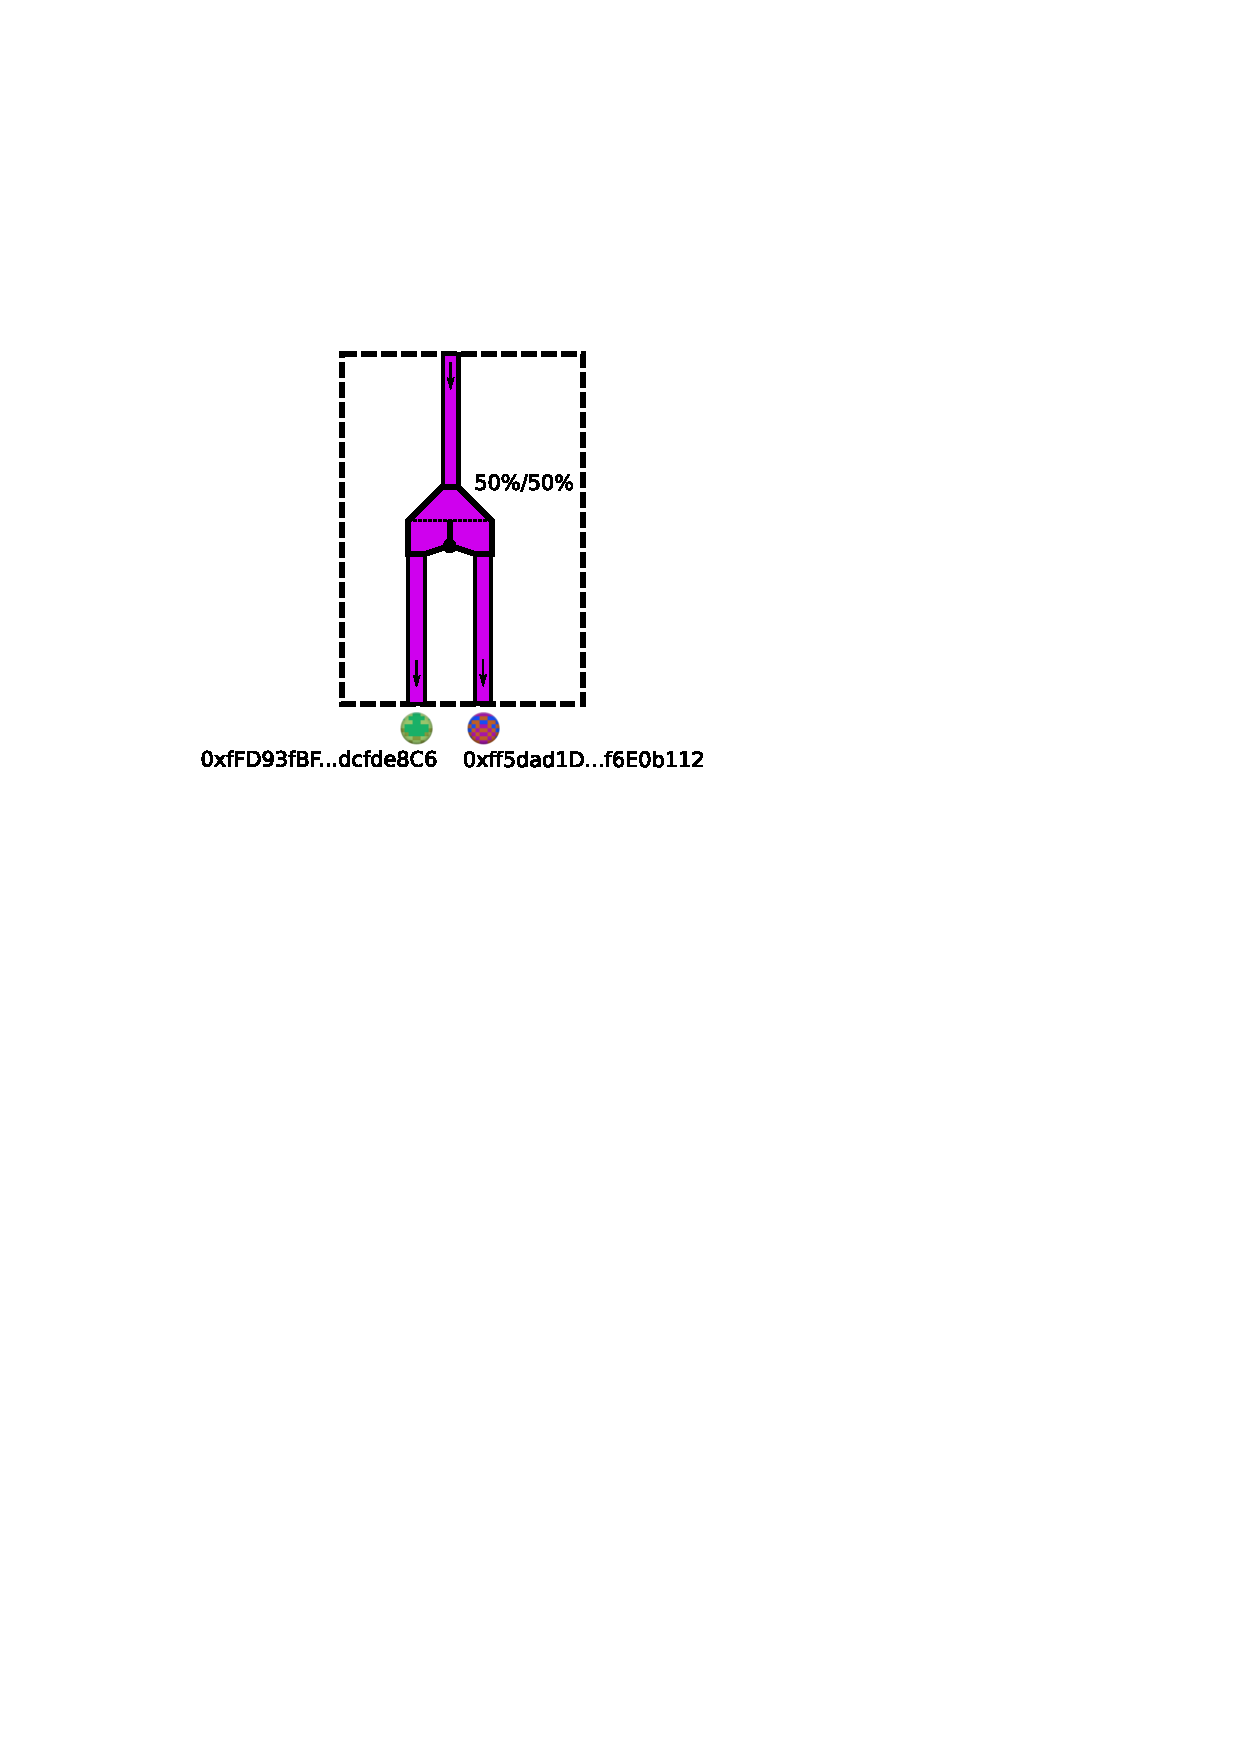
\includegraphics[height=4cm]{splitter.pdf}
\caption{Smart contract that distributes all Ether sent to it equally among
two addresses.}
\label{splitter}
\end{figure}

Let us now look at an extension of this simple splitter, the adjustable splitter,
which can be seen in Figure \ref{adjustable_splitter}.
This contract has a small button or lever at the outside and an address
written next to it telling that only this address is allowed to manipulate the
button.

\begin{figure}
\center
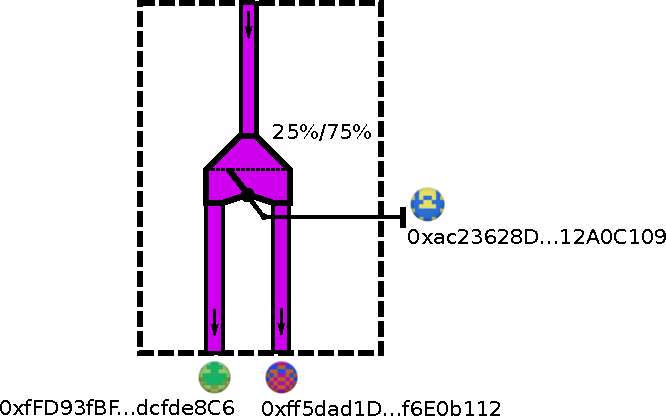
\includegraphics[height=4cm]{adjustable_splitter.pdf}
\caption{Smart contract that distributes all Ether sent to it among
two addresses with a ratio modifiable from a certain address.}
\label{adjustable_splitter}
\end{figure}

The basic idea of Babbage is to provide multiple ``gadgets'' that can be
combined with each other, but only ``snap'' together in certain combinations.
The final smart contract that is executed on the Ethereum Virtual Machine
will of course not do a full physics simulation as that would be too expensive.
Instead, the IDE will translate gadget combinations into smart contract code.
At the same time, the IDE will make sure that unintended physical interactions
like collisions between moving rods or levers are not possible. This is important
since such collisions
would not be modeled by the smart contract, but at the same time,
humans looking at the diagram could expect them to actually happen.
In general, all gadgets should be
as simple and intuitive as possible. The examples provided in this document probably
do not yet achieve the desired level of simplicity, but they provide a
perspective on the general idea.

The adjustable splitter might be translated into the following code:

{
\small
\begin{verbatim}
pragma solidity ^0.4.10;
contract AdjustableSplitter {
  uint splitter_setting = 25;
  address controller = 0xac23628D25A36ba7834fd171Dc3F794F12A0C109;
  address exit1 = 0xfFD93fBFA184B6dfaaA8684B97Ec3F71dcfde8C6;
  address exit2 = 0xff5dad1Db92AF1987A10Fc62D2B93F14f6E0b112;

  function receiveEther() payable {
    splitter_etherInjected(msg.value);
  }

  function splitter_etherInjected(uint amount) internal {
    uint setting = splitter_setting;
    uint amount_toLeft = amount * setting / 100;
    pipe1_etherInjected(amount_toLeft);
    pipe2_etherInjected(amount - amount_toLeft);
  }

  function splitter_adjustSetting(uint setting) internal {
    require(setting <= 100);
    splitter_setting = setting;
  }

  function pipe1_etherInjected(uint amount) internal {
    exit1.transfer(amount);
  }

  function pipe2_etherInjected(uint amount) internal {
    exit2.transfer(amount);
  }

  function rod1_moved(uint toSetting) {
    require(msg.sender == controller);
    splitter_adjustSetting(toSetting);
  }

  function() payable {
    receiveEther();
  }
}
\end{verbatim}
}

The final example in Figure \ref{escrow} shows an escrow contract.
The idea behind this mechanism is that one person, Alice, wants to sell
an item to another person, Bob. The payment should happen via the Ethereum
network, but the item has to be sent via parcel from Alice to Bob.
Alice deposits the value of the item into the smart contract. As long
as Bob does not yet do the same, Alice can still drain the contract.
Once Bob put his Ether in, the contract is locked in the following sense:

The only option available to Bob is to trigger a mechanism in the contract
that will send all Ether in the contract to Alice. Bub would use this
when he receives the item and thus performs the final payment.

The only option for Alice is to trigger a mechanism that will refund both
Alice and Bob. This should be used in a situation where something went wrong
with the parcel or Bob returned the item.

When analyzing the diagram, note that Ether always flows according to the arrows
and if an interaction with a smart contract
triggers something inside the contract to move (or flow), the next interaction
is only possible once everything stopped moving. Furthermore, pipes cannot
store Ether (you can think of pipes as not having any internal volume),
so Ether either has to move through the pipes completely and end up in some
kind of reservoir or not enter the pipes at all. Red wires can carry single
impulse signals and only in the direction indicated by the arrows.

\begin{figure}
\center
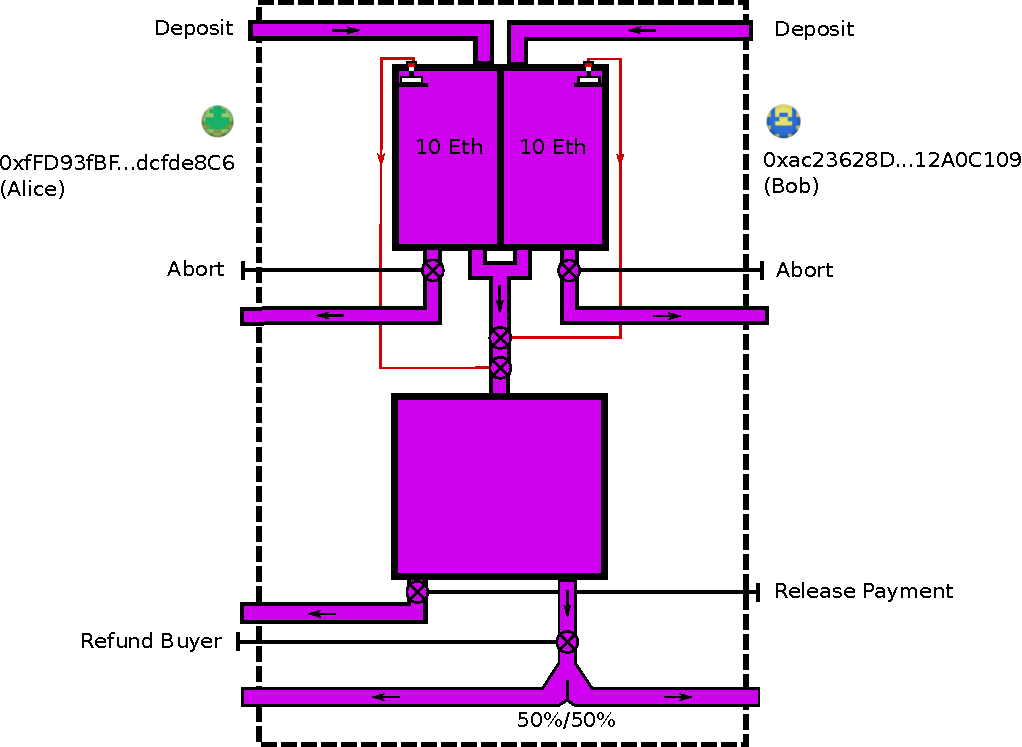
\includegraphics[width=12cm]{escrow.pdf}
\caption{Escrow mechanism that first requires two parties to deposit the same
amount of Ether and then allows payouts to be performed in different ways
by the parties. The circles are valves that change their opened / closed
state by actuating them and the gadgets at the top of the tanks are
float switches.}
\label{escrow}
\end{figure}

Let us go through the full escrow mechanism. In the top-center we have two
identical tanks that can both store 10 Ether. Each of the tanks has two
drains which are closed by valves in the beginning. Both Alice and Bob can
open their valve and get their Either back. At the top of each tank
is a float switch that activates a signal that travels along the red wires
to a valve at the center drain pipe. This mechanism ensures that as soon as
both tanks are filled, they are automatically drained into the bottom tank.
Note how the two sequential valves act as an ``and'' gadget. Also note that
both of the tanks can be filled and drained multiple times as long as the
other tank is not completely filled.

Once the Ether reached the second tank, Alice only has the option to open
the valve attached to the right drain pipe and refund both Alice and Bob.
On the other hand, Bob only has the option to open the left valve, thus
sending all Ether to Alice and paying for the purchase this way.

One thing that is immediately obvious from the diagram is the symmetry of
interaction between the parties. Everything is fully symmetric apart from
the actual ``payout'' section. For textual programming languages, such
properties are only visible after careful inspection of the source code.
\end{document}
